\documentclass{standalone}
\usepackage{tikz}
\usepackage{ctex,siunitx}
\setCJKmainfont{Noto Serif CJK SC}
\usepackage{tkz-euclide}
\usepackage{amsmath}
\usetikzlibrary{patterns, calc}
\usetikzlibrary {decorations.pathmorphing, decorations.pathreplacing, decorations.shapes,}

\begin{document}
\small
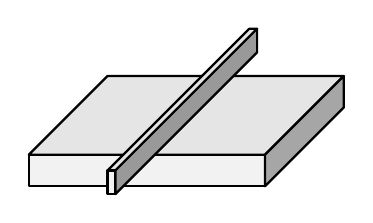
\begin{tikzpicture}[>=stealth,scale=1.0,line join=round]
  \tkzSetUpPoint[fill=black]
  % \useasboundingbox(-1,-0.75)rectangle(3.7,1.4);
  \tkzDefPoints{0/0/A,3/0/B,4/1/C,1/1/D,0/-0.4/A'}
  \tkzDefPoints{1/-0.2/O,1.1/-0.2/P,2.9/1.6/Q,2.8/1.6/R,1/-0.5/O'}
  \tkzDefPointsBy[translation = from A to A'](B,C){B',C'}
  \tkzDefPointsBy[translation = from O to O'](P,Q){P',Q'}
  \draw[thick,fill=gray!20](A)--(B)--(C)--(D)--cycle;
  \draw[thick,fill=gray!10](A)--(A')--(B')--(B)--cycle;
  \draw[thick,fill=gray!70](B')--(B)--(C)--(C')--cycle;
  \draw[thick,fill=gray!20](O)--(P)--(Q)--(R)--cycle;
  \draw[thick,fill=gray!10](O)--(O')--(P')--(P)--cycle;
  \draw[thick,fill=gray!80](P')--(P)--(Q)--(Q')--cycle;
\end{tikzpicture}
\end{document}